\documentclass{standalone}
\usepackage{tikz}

\begin{document}

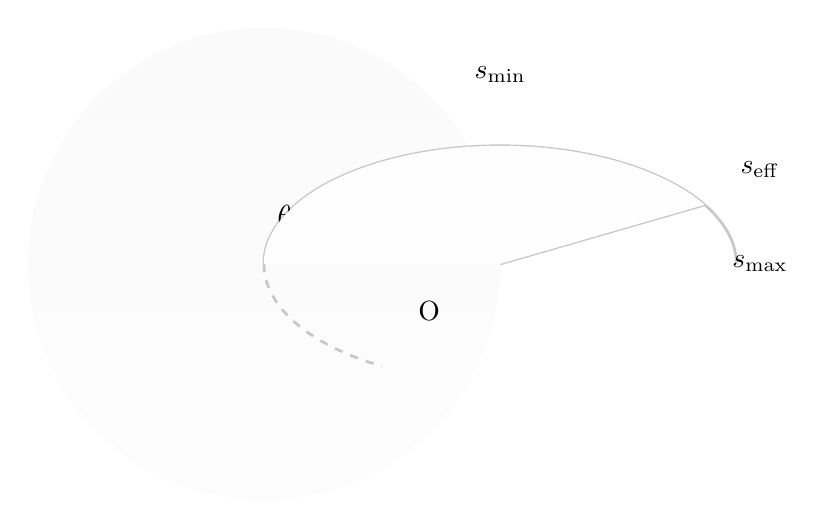
\begin{tikzpicture}[scale=3]
    % Define colors
    \definecolor{sphereColor}{RGB}{250,250,250}
    \definecolor{lineColor}{RGB}{200,200,200}
    
    % Draw the sphere
    \shade[bottom color=sphereColor!50, top color=sphereColor] (-1,0) circle (1);
    
    % Draw the spherical cap
    \draw[line width=1pt, lineColor] (-1,0) arc (180:0:1 and 0.5);
    \draw[dashed, line width=1pt, lineColor] (-1,0) arc (180:360-120:1 and 0.5);
    \draw[dotted, line width=1pt, lineColor] (-1,0) arc (180:360-180:1 and 0.5);
    
    % Draw the dashed line representing s_{\mathrm{eff}}
    \draw[dashed, line width=1pt, lineColor] (0,0) -- (70:1 and 0.5);
    
    % Draw the solid lines representing s_{\mathrm{min}} and s_{\mathrm{max}}
    \draw[line width=1pt, lineColor] (0,0) -- (90:1 and 0.5);
    \draw[line width=1pt, lineColor] (0,0) -- (30:1 and 0.5);
    
    % Add labels
    \node at (0, 0.8) {$s_{\mathrm{min}}$};
    \node at (1.1, 0.4) {$s_{\mathrm{eff}}$};
    \node at (1.1, 0) {$s_{\mathrm{max}}$};
    \node at (-0.3, -0.2) {O};
    \node at (-0.8, 0.2) {$\theta_{\mathrm{MAX}}$};
    
    % Add the shaded regions
    \fill[sphereColor!30] (0,0) -- (90:1 and 0.5) arc (90:30:1 and 0.5);
    \fill[sphereColor!30] (0,0) -- (90:1 and 0.5) arc (90:180:1 and 0.5);
    
\end{tikzpicture}

\end{document}